\documentclass[a4paper,10pt]{article}

\usepackage[margin=3cm]{geometry}
\usepackage[pdftex]{graphicx}
\usepackage{verbatim,url}

\begin{document}

\title{
  {\normalsize
    Introduction to Algorithms, Data Structures, and Problem Solving\\
    DA4002 (HT11) Halmstad University}\\
  Example Report with Guidelines\\
  Project 1: Computational Complexity
}
\author{
  Roland Philippsen\\
  course examiner\\
  \texttt{roland.philippsen@hh.se}
}
\maketitle



\section{Introduction}

A (short!) written report is an essential part of the project.
It must clearly identify the team and present the work performed by them.
This example report provides a recommended format.

The introduction is the place to introduce the problem and briefly state what results have been achieved.
For project 1, this means stating which benchmark problem you have chosen to solve.
You should also briefly explain how far you have advanced through the mandatory tasks (this can be as simple as saying ``all mandatory tasks have been done''),
and whether you have done any bonus tasks.

In case you hand in a partial solution, this should already be mentioned in the introduction, but details should wait until the implementation or results section.
If you need rather long explanations for some of these aspects, you can put that into a separate discussion section.

This example report uses the two benchmark applications given to the course participants as technical examples.
It presents how to run the benchmarks and the basic plots that can be produced.



\section{Implementation}

The implementation section should introduce any new sources, classes, and methods.
You should also explain how you have integrated your changes into the benchmark.

For example, if you have chosen alternative B and implemented \emph{bubble sort}~\cite{wikipedia:bubble-sort}, you could write something like this:
``The source file \texttt{BubbleSort.java} contains a class called \texttt{BubbleSort} which has a method called \texttt{sort} that sorts a given array of strings using the bubble sort algorithm.
The implementation is based on the pseudo-code shown in figure~\ref{fig:bubble-sort}.''

\begin{figure}
  \centering
  \fbox{
    \begin{minipage}{0.7\columnwidth}
      \verbatiminput{bubble-sort.txt}
  \end{minipage}}
  \caption{
    Pseudo-code for bubble sort, taken from Wikipedia~\cite{wikipedia:bubble-sort}.
  }\label{fig:bubble-sort}
\end{figure}

As you can see, it is acceptable to copy-paste \emph{short} sections from other sources, such as websites or books, \emph{as long as} this is properly marked as a quotation and the original source is given.
Note that bubble sort is \emph{not} on the list of algorithms you can choose for the mandatory tasks of alternative B, because bubble sort has already been done during exercise 3.5.

The two example benchmark applications that are provided as starting points for the first ITADS project are partially based on source code that was already seen during exercises.
In general, source file names match class names, so \texttt{ExampleA.java} contains class \texttt{ExampleA} which has a \texttt{main} method that measures the runtime of inserting items into a list and a vector.
\texttt{ExampleB.java} is very similar, except that it measures the time it takes to sort arrays of random strings with the merge and insertion sort algorithms.
Both these examples rely on utilities and other classes implemented in the other files that come bundled in the source archive for project 1:

\begin{itemize}

\item
  \texttt{Factory.java} contains a class which provides methods for generating input data.
  Most importantly, the \texttt{createRandomStrings} method creates an array of $N$ strings.
  Each string in that array will be between 2 and 11 characters long, and it is composed of random alphanumeric characters.
  The other methods are \texttt{createSamples} (which is useful for some of the bonus tasks), various \texttt{duplicate} methods, and a short \texttt{main} which serves as demo.

\item
  \texttt{LogEntry.java}, \texttt{LogSeries.java}, and \texttt{LogBook.java} contain classes
  that log the benchmark data and produce the files and plot scripts that can be used to create figures for presenting your results.
  The most important methods are the following:
  \begin{itemize}
  \item
    \texttt{LogBook.addSeries} defines a new \texttt{LogSeries} instance to be added to the log.
  \item
    \texttt{LogBook.createFiles} writes all data of all registered \texttt{LogSeries} objects, and also creates plot script files that reference these log data files.
  \item
    \texttt{LogSeries.startSingle} and \texttt{LogSeries.stopSingle} are used to record a single data point.
  \end{itemize}
  The \texttt{main} methods of the \texttt{ExampleA} and \texttt{ExampleB} classes clearly illustrate how to use the logging facilities.

\item
  \texttt{StringList.java}, \texttt{StringListIterator.java}, \texttt{StringListNode.java}, and \texttt{String\-Vector\-.java} contain classes which implement the doubly-linked list and the dynamically growing array that have been developed during exercise 2.

\item
  \texttt{InsertionSort.java} and \texttt{MergeSort.java} contain the classes which implement the sorting algorithms used by \texttt{ExampleB}.
  Both of them contain a \texttt{sort} method which applies insertion sort~\cite{wikipedia:insertion-sort} and merge sort~\cite{wikipedia:merge-sort}, respectively, on an array of strings.

\end{itemize}

Another important thing to explain in the implementation section is how to compile and run the applications that you have written.
The code provided as starting point of the project is compiled using the \texttt{make} command, which invokes GNU Make~\cite{gnu-make}.
This will read build instructions from the \texttt{Makefile} which is part of the sources, and create \texttt{.class} files for all the \texttt{.java} files in the directory.

Running the example applications is simply a matter of passing their class names to the \texttt{java} virtual machine.
This is done by opening a terminal and giving the following commands:

\begin{verbatim}
java ExampleA
java ExampleB
\end{verbatim}

Running \texttt{ExampleA} produces console output like the one in figure~\ref{fig:exa-console}.
And \texttt{ExampleB} is very similar, as can be seen in figure~\ref{fig:exb-console}.

\begin{figure}
  \centering
  \fbox{
    \begin{minipage}{0.8\columnwidth}
      \verbatiminput{console-ExampleA.txt}
  \end{minipage}}
  \caption{
    Typical console output from \texttt{ExampleA}.
    The table with the running times gives feedback while the benchmark is being run.
    The list of commands at the end allows to view and create figures.
  }\label{fig:exa-console}
\end{figure}

\begin{figure}
  \centering
  \fbox{
    \begin{minipage}{0.8\columnwidth}
      \verbatiminput{console-ExampleB.txt}
  \end{minipage}}
  \caption{
    Typical console output from \texttt{ExampleB}.
    Similarly to figure~\ref{fig:exa-console}, the table is produced while the benchmark is being run.
    Again, the list of commands at the end allows to view and create figures.
  }\label{fig:exb-console}
\end{figure}

In case you hand in some partially solved tasks which do not compile, this should be clearly explained: which file does not compile, and why?
What would need to be done in order to make it compile?
Any compilation errors that are not covered by such an explanation are a serious failure.

In a more general sense, when writing applications that must be used by others (who may not be programmers, or who may not have access to the source code), the explanations you write here are the only way for people to find out how to use your application.
For this project, it is enough to give the exact command required to produce each figure in the results section, and you can do that inside the results section.
If your code produces some special output on the terminal which is needed to understand your results, then you should also include some example output and explain which part is special, and why.



\section{Results}

In the results section, you have to present the obtained technical results.
For the first project, this means that for each task, you have to produce one or more figures which clearly illustrate the point you are making.
For example, if you found out that the running time of a sorting algorithm gets much worse if the input data is in reverse-sorted order, then you have to include a figure which shows just this effect.
It is also important to summarize your main findings in order to give a high-level understanding.
This can be done at the end of the results section, or in a separate discussion or conclusion.
Sometimes, it also makes sense to additionally (and very briefly) mention your main result already in the introduction.

The two example applications produce data and plot files that are ready to use.
\texttt{ExampleA} produces plots such as the one shown in figure~\ref{fig:exa-plot}.
This figure shows that the insertion times for lists and vectors are quite short.
It also shows that the variation in the measurement can be quite high.
This makes it hard to see that the running time actually follows an $O(N)$ complexity curve.
After you have performed the third mandatory task, these plots should produce somewhat smoother curves.

\begin{figure}
  \centering
  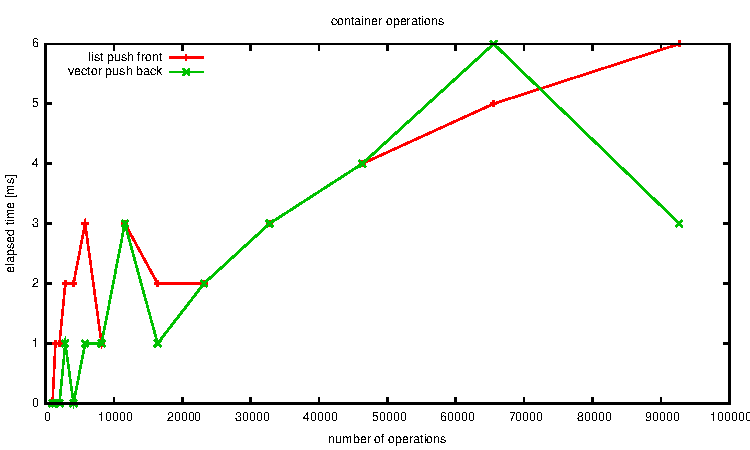
\includegraphics[width=0.8\columnwidth]{plot-ExampleA.pdf}
  \caption{
    Execution time plot produced by running example A, and then using the automatically generated plot script like this:
    ``\texttt{gnuplot log-1316350931155-all-pdf.plot}''
  }\label{fig:exa-plot}
\end{figure}

\texttt{ExampleB} measures the running time of insertion and merge sort.
As shown in figure~\ref{fig:exb-plot}, there is a significant difference between these two algorithms.
Insertion sort is known to be $O(N^2)$~\cite{wikipedia:insertion-sort} and this fits qualitatively.
Of course, a proper empirical analysis would have to include a more precise technical demonstration of whether the measured running times actually follow a quadratic curve.
This was presented during lecture 4, and is one of the bonus tasks available for alternative B.

Another important point visible in figure~\ref{fig:exb-plot} is that merge sort is much faster than insertion sort.
So, figure~\ref{fig:exb-merge-plot} shows just the data of merge sort.
From that figure it would be hard to see that merge sort is $O(N\log N)$~\cite{wikipedia:merge-sort}.
One reason is that the benchmark was not pursued for large enough problem sizes, and another one is the ``noise'' for very small problems.
These kinds of issues can be addressed in a bonus task.
For instance by creating a separate benchmark which looks just at merge sort (and maybe other $O(N\log N)$ sorting algorithms) over a larger range of problem sizes, and matching it with the theoretical growth curves.

\begin{figure}
  \centering
  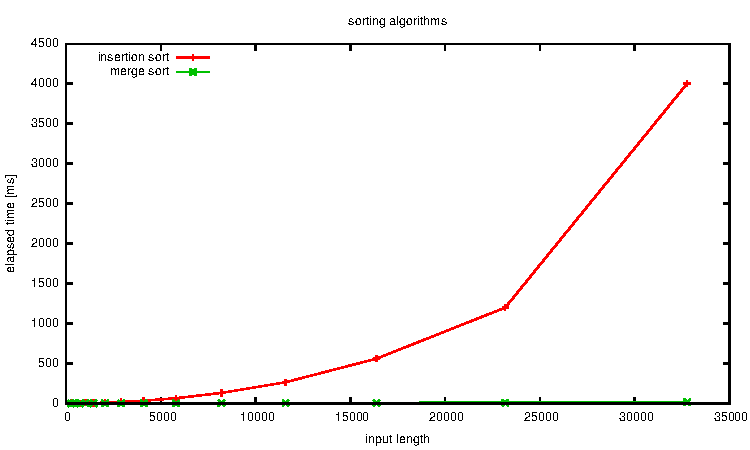
\includegraphics[width=0.8\columnwidth]{plot-ExampleB-all.pdf}
  \caption{
    Execution time plot produced by running example B.
    Merge sort is so fast that its running time graph almost coincides with the X axis.
  }\label{fig:exb-plot}
\end{figure}

\begin{figure}
  \centering
  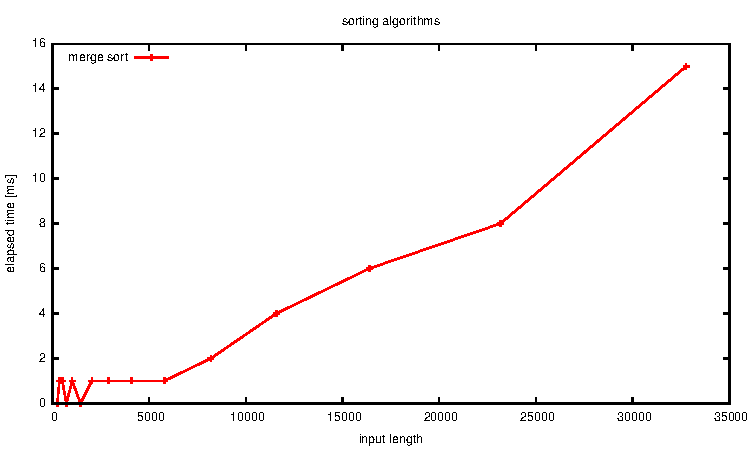
\includegraphics[width=0.8\columnwidth]{plot-ExampleB-zoom.pdf}
  \caption{
    Execution time plot of merge sort.
  }\label{fig:exb-merge-plot}
\end{figure}

Summarizing the results of running the example benchmarks, it can be said that they give a good starting point for further work.
The data they produce is a bit too noisy, and they do not compare enough different algorithms and data structures to make really general statements.
But if they did that, then the course participants would have nothing to do during their projects\ldots



\section{Further Remarks}

As explained during lecture 4, the submission format for the projects is as follows:\\
-- Submit either individual files, or a ZIP or TAR archive.\\
-- All Java source code must be handed in.\\
-- The report must be in PDF format.\\
-- Everything has to be sent via email to the course examiner by Friday, September 30, at 18h.\\

The ITADS course focuses on technical aspects of programming and problem solving.
The quality of the written language in the report is secondary.
As long as it remains comprehensible, English errors are not relevant.
Verbatim quotes (copy-pasting) from other sources is acceptable \textbf{if they are short, properly marked, and adequately cited}.

If language is a major obstacle for a team, it is possible to receive a deadline extension for the report only.
Source code will still have to be handed in at the normal deadline.
Notify the lecturer as early as possible in order to arrange a deadline extension for the report.

Halmstad University offers an \textbf{English Language Studio} for students who seek help with written English.
The studio is available on Wednesdays between 9:00 and 12:00 in room F-208.
The teacher is Nicholas Lloyd-Pugh \texttt{<nicholas.lloyd-pugh@hh.se>} (phone 167372).



\section{Conclusion}

The most important points to remember about the report are:

\begin{itemize}
\item Mention course information: University name; course name, code, and date.
\item Mention team information: names, email addresses, and study programme.
\item Don't forget the project title and subtitle.
\item The introduction section must summarize the work you have done.
\item The implementation must present what you have added and changed, and how to run it
\item the results must clearly show what you have achieved
\item a separate discussion section is possible if you want to give a high-level explanation of the detailed technical results
\item a conclusion is also a nice additional section, it allows you to make some overall comments and maybe point to future work
\item references must be given to all the web sites, books, and other material that you have used\footnote{
  except the most obvious sources, such as the course book or the lecture slides};
  it is acceptable to quote (copy-paste) those sources, as long as the quotes are short, clearly marked, and properly referenced
\end{itemize}

This example report mixes technical aspects and general writing guidelines.
Your project report will probably be much shorter, which is just fine (and less work for the evaluation).
Good luck with your work!



\bibliographystyle{plain}
\bibliography{itads-bibliography}

\end{document}
